%%
%% Copyright 2007, 2008, 2009 Elsevier Ltd
%%
%% This file is part of the 'Elsarticle Bundle'.
%% ---------------------------------------------
%%
%% It may be distributed under the conditions of the LaTeX Project Public
%% License, either version 1.2 of this license or (at your option) any
%% later version.  The latest version of this license is in
%%    http://www.latex-project.org/lppl.txt
%% and version 1.2 or later is part of all distributions of LaTeX
%% version 1999/12/01 or later.
%%
%% The list of all files belonging to the 'Elsarticle Bundle' is
%% given in the file `manifest.txt'.
%%

%% Template article for Elsevier's document class `elsarticle'
%% with numbered style bibliographic references
%% SP 2008/03/01
%%
%%
%%
%% $Id: elsarticle-template-num.tex 4 2009-10-24 08:22:58Z rishi $
%%
%%
\documentclass[preprint,12pt,3p]{elsarticle}

%% Use the option review to obtain double line spacing
%% \documentclass[preprint,review,12pt]{elsarticle}

%% Use the options 1p,twocolumn; 3p; 3p,twocolumn; 5p; or 5p,twocolumn
%% for a journal layout:
%% \documentclass[final,1p,times]{elsarticle}
%% \documentclass[final,1p,times,twocolumn]{elsarticle}
%% \documentclass[final,3p,times]{elsarticle}
%% \documentclass[final,3p,times,twocolumn]{elsarticle}
%% \documentclass[final,5p,times]{elsarticle}
%% \documentclass[final,5p,times,twocolumn]{elsarticle}

%% if you use PostScript figures in your article
%% use the graphics package for simple commands
%% \usepackage{graphics}
%% or use the graphicx package for more complicated commands
%% \usepackage{graphicx}
%% or use the epsfig package if you prefer to use the old commands
%% \usepackage{epsfig}

%% The amssymb package provides various useful mathematical symbols
\usepackage{amssymb}
\usepackage{amsmath}
%% The amsthm package provides extended theorem environments
\usepackage{amsthm}
\usepackage{times} % assumes new font selection scheme installed
\usepackage{graphics} % for pdf, bitmapped graphics files
\usepackage{float}
\usepackage{xcolor}
\definecolor{verde}{rgb}{0,0.5,0}
\usepackage{verbatim}

\usepackage{listings}
\lstset{
    %frame=tb, % draw a frame at the top and bottom of the code block
    tabsize=4, % tab space width
    showstringspaces=false, % don't mark spaces in strings
    numbers=left, % display line numbers on the left
    %commentstyle=\color{verde}, % comment color
    %keywordstyle=\color{blue}, % keyword color
    %stringstyle=\color{red} % string color
	belowcaptionskip=1\baselineskip,
	breaklines=true,
	frame=false,
	xleftmargin=\parindent,
	basicstyle=\scriptsize\ttfamily,
	%basicstyle=\footnotesize\ttfamily, %edit to get bigger font
	keywordstyle=\bfseries\color{green!40!black},
	commentstyle=\itshape\color{purple!40!black},
	identifierstyle=\color{blue}, %functions
	stringstyle=\color{orange},
}
\lstnewenvironment{ttlisting}{\lstset{ 
	basicstyle=\scriptsize\ttfamily\color{black}, identifierstyle=\color{darkgray},}}{}
%% The lineno packages adds line numbers. Start line numbering with
%% \begin{linenumbers}, end it with \end{linenumbers}. Or switch it on
%% for the whole article with \linenumbers after \end{frontmatter}.
\usepackage{lineno}

%% natbib.sty is loaded by default. However, natbib options can be
%% provided with \biboptions{...} command. Following options are
%% valid:

%%   round  -  round parentheses are used (default)
%%   square -  square brackets are used   [option]
%%   curly  -  curly braces are used      {option}
%%   angle  -  angle brackets are used    <option>
%%   semicolon  -  multiple citations separated by semi-colon
%%   colon  - same as semicolon, an earlier confusion
%%   comma  -  separated by comma
%%   numbers-  selects numerical citations
%%   super  -  numerical citations as superscripts
%%   sort   -  sorts multiple citations according to order in ref. list
%%   sort&compress   -  like sort, but also compresses numerical citations
%%   compress - compresses without sorting
%%
%% \biboptions{comma,round}

% \biboptions{}


\journal{Harvard Biorobotics Lab}

\begin{document}

\begin{frontmatter}

\title{ Improving end joint sensing for robotic grasping\\
(Using IMUs to estimate contact force) }

%\tnotetext[label0]{This is only an example}

\author{Final report for Spring 2018 rotation in Harvard Biorobotics Lab\\
~\\
Nao Ouyang}
%\address[label1]{Address One}

%\address[label2]{Address Two\fnref{label4}}
%\author[label1,label2]{Author One\corref{cor1}\fnref{label3}}
%\address[label1]{Address One}
%\address[label2]{Address Two\fnref{label4}}

%\cortext[cor1]{I am corresponding author}
%\fntext[label3]{I also want to inform about\ldots}
%\fntext[label4]{Small city}

%\ead{author.one@mail.com}
%\ead[url]{author-one-homepage.com}

%\author[label5]{Author Two}
%\address[label5]{Some University}
%\ead{author.two@mail.com}

%\author[label1,label5]{Author Three}
%\ead{author.three@mail.com}

\begin{abstract}
    Despite decades of research, robots remain unable to reliably grasp objects in environments not
    designed for robots. Thus, they are not able to work alongside us in human environments or
    outside buildings. One approach is to use tactile sensing to predict whether a
    grasp will succeed or not as well as build simulations to evaluate potential grasps.
    In this lab, we use an underactuated three-fingered gripper, which makes it difficult to
    estimate the location of the fingers and and the location of the force with respect to the robot
    frame of reference.  \\
    I investigated the use of an inertial measurement unit to provide such information. By
    characterizing the stiffness matrix $K$ of the finger, I could investigate whether using an
    inexpensive inertial measurement unit (IMU) to estimate $\theta$ deflection with the linear equation
    $\tau = K \theta$, I could discover information about the force applied. I did very preliminary
    work, limiting my experiments to the case where we only desire to estimate the change from
    directly before to second or two after
    contact. Additionally, I looked at using of off-the-shelf machine learning approaches to reduce the
    errors in our model. Finally, I investigated adding more sensors to the fingertip in
    order to better estimate contact location. 
\end{abstract}



\end{frontmatter}

%%
%% Start line numbering here if you want
%%
% \linenumbers

%% main text


\section{Introduction}
State-of-the art robots are bad at grasping in unstructured environmnents, limiting their use to
structured environments like factory floors. An active area of research in order for robots to expand to unstructured
environments (such as kitchens or hospital environments),  is the ability to grasp
novel objects (objects the robot has not encountered before and may not have any prior information
about). Grasp stability analysis plays a critical role in enabling robots to achieve high grasping
success rates (in terms of not dropping objects). Through sensing, for instance tactile sensing, we
can predict whether or not we will drop the object after grasping and prior to moving. If we find
our grasp to be unstable, and assuming the object has not moved during grasping such that releasing
our grip might e.g. cause it to tumble, we can simply release our grasp and try again. 

Physical model approaches involve modeling the contact forces, contact location, and surface normals
(which will differ from the force XYZ if the surface(s) are squishy).  However, over the last few
decades physical models have proven insufficient. This in part due to complex gripper-object
interactions during grasping which are both difficult to measure and hard to model. Thus, one of the
aspects of this investigation is to evaluate whether machine learning can be used to improve
physical models. We can combine the good aspects of physical models (good generalizability,
requiring significantly less data than in pure computer vision machine learning approaches) with
(not having to have extremely precise models). I tried to charactize the residuals in
the physical models and determine if these residuals could be more accurately modelled by a black
box machine learning approach rather than making the physical model more complex. This is an
increasingly popular approach, which makes intuitive sense. We can leverage
domain knowledge, instead of using an end-to-end approach for sensor data to stability prediciton.

Although there are a few compact 6 axis force torque sensors, they cost multiple thousands of
dollars and are finicky and fragile. Thus, we would like to use an inexpensive nine
degree-of-freedom (three-axis acceleromter, gyrometer, and magnetic heading) IMU instead.

During the course of this rotation, senior graduate student Qian Wan discoverd that the current tactile
sensors are insufficent for estimating contact location accurately enough to develop a good grasp
stability estimate. Thus, this project includes a brief exploration of a new sensor design using the
same elements (barometric pressure sensors covered by a layer of elastomer, such as urethane), but
more of them.

\section{Theory} \label{sec:firstpage}


\subsection{Model}

For the model, we are making a few simplifying assumptions:

1. There is a linear relationship between force and deflection, or alternatively torque and angle of
deflection
2. The center of the axis of rotation was at the tip of the proximal joint
(in reality, likely it is two or three mm shifted outward, and changes as the flex increases)
3. We consider the z axis to be defined respect to the surface of the finger, so that z=0 is always
at the tip of the finger

The consequence of \#3 is that we cannot estimate z-axis torque.

\subsection{Reference Frame}

\begin{ttlisting}[language=C++,breaklines]
Coordinates
----> + x (roll)
|
|
v
+ y (pitch)

+ z (up out of page) (yaw)


Finger Positions
=======      ====================.
 {CL}  || --- || 15  12  9  6  3 ||
 {A} [xy=0]-- || 14  11  8  5  2 ||
 {MP}  || --- || 13  10  7  4  1 ||
=======      ====================.


  [[---]]
||  WEB  ||
||  CAM  ||
  ||--- ||
  
Points 13 through 15 are at x=2.6 cm, and each x is spaced 5 mm apart.
\end{ttlisting}


\subsection{Linear Model, 1D case}

In the one-axis case, the math is straightforward.

\begin{align}
\tau = k \times F
\end{align}

For example, one datapoint might be

\begin{align}
k &= F / \tau \\
k &= (20g \times 9.8 m/s^2)/0.1 \text{ degrees}
\end{align}

where `k` represents the stiffness of the finger. Let $c$ represent the inverse of $k$.

Using least squares error, we may fit a line to find $\hat{c}$. 

\begin{align}
 \hat{c} &= \frac{1}{\hat{k}} \\
 \theta &= \tau \hat{c} + b
\end{align}

where $b$ be a constant determined by the line of fit.



\subsection{Residuals}

From the above, we may calculate the residuals of any of our estimated variables.
For instance, from our actual data we may obtain an estimate for `k`.

\begin{align}
 \tau_{data} &= \hat{k} \cdot \theta_{data} \\
\end{align}

Using this k we can go back and calculate estimates for the "true" torque, assuming our linear model was correct.

\begin{align}
 \hat{\tau} &= \hat{k} \cdot \theta_{data} 
\end{align}

We would then calculate our torque residuals as

\begin{align}
 \epsilon_{\tau} = \hat{\tau} - \tau 
\end{align}

If we plot a graph of (torque residuals) vs (estimate residuals) and find that our points are randomly scattered around a straight line, then our model well-approximates reality as sensed by a noisy sensor.

However, our residuals may instead follow a parabola, in which case we would want to amend our model
to have higher-order terms.

\begin{align}
 \hat{\tau} = \hat{k}\theta_{data} +c_1 \theta_{data} + c_2 \theta_{data}
\end{align}

and so forth. 

We may eventually use machine learning techniques to fit higher-order terms.

\subsection{3D case}
The 3d case is exactly the same, except now each of the variables are vectors or matrices. 

    %:s@\\\[:\\begin{bmatrix}:g
\begin{align}
    \begin{bmatrix} \vec{\tau} \end{bmatrix}_{3\times n}  = \begin{bmatrix} K \end{bmatrix}_{3\times 3} \cdot \begin{bmatrix} \vec{\theta} \end{bmatrix}_{3\times n} 
\end{align}

where

\begin{align}
\vec{\tau} &= \begin{bmatrix} \stackrel{3\times 1}{\tau_1} | \stackrel{3\times 1}{\tau_2} | ... |\stackrel{3\times 1}{\tau_n} \end{bmatrix} \\
\\
\vec{\theta} &= \begin{bmatrix} \stackrel{3\times 1}{\theta_1} | \stackrel{3\times 1}{\theta_2} | ... |\stackrel{3\times 1}{\theta_n} \end{bmatrix}
\end{align}

\subsection{Sanity Check: Simplify to 2D case}

We know that $\tau = r \times F$

\begin{align}
    \begin{bmatrix}
        \tau_{x} \
        \tau_{y} \
        \tau_{z} \
    \end{bmatrix} =
    \Bigg[ \; K \; \Bigg]_{3\times3} \;
    \begin{bmatrix}
        \theta_{x} \
        \theta_{y} \
        \theta_{z} \
    \end{bmatrix} \
\end{align}

Further, we can use some of the simplifying assumptions we made about to model our system, in order to have an idea of what values our math should result in for $k$.

We may also see that we will only ever have x and y components for $r$; z components for $F$; and thereforce (by how cross products work) only ever have x and y components for $\tau$.

\textbf{Off-axis}
\begin{align}
r \approx
\begin{bmatrix}
    r_x       \\
    r_y       \\
    0       \\
\end{bmatrix} \; \times \;
f \approx
\begin{bmatrix}
    0       \\
    0       \\
    f_z      \\
\end{bmatrix} \; =  \; \tau \; = 
\begin{bmatrix}
    \tau_x       \\
    \tau_y       \\
    0      \\
\end{bmatrix}\\
\end{align}


\textbf{On-Axis}

In the even more simplified case, if we do not apply the force off-axis and there is only a pitch
deflection

\begin{align}
r \approx
\begin{bmatrix}
    r_x       \\
    0       \\
    0       \\
\end{bmatrix} \; \times \;
f \approx
\begin{bmatrix}
    0       \\
    0       \\
    f_z      \\
\end{bmatrix} \; =  \; \tau \; = 
\begin{bmatrix}
    0 \\
    \tau_y       \\
    0      \\
\end{bmatrix}\\
\end{align}

We \textbf{could} have enough nonzero values for the xyz components of $\theta$ that we will be able
to calculate a nondegenerate estimate for $k$. This is thanks to applying the force off-axis,
causing the finger to roll and create non-zero elements for $\theta_y$ ( our roll) and $\theta_z$
(our yaw). However, after solving for K, I found that I ended up with a bottom row consisting
entirely of zeroes.

Here is a well-formatted version on Wikipedia describing the 3D stiffness tensor. 

\begin{figure}[H]
\centering
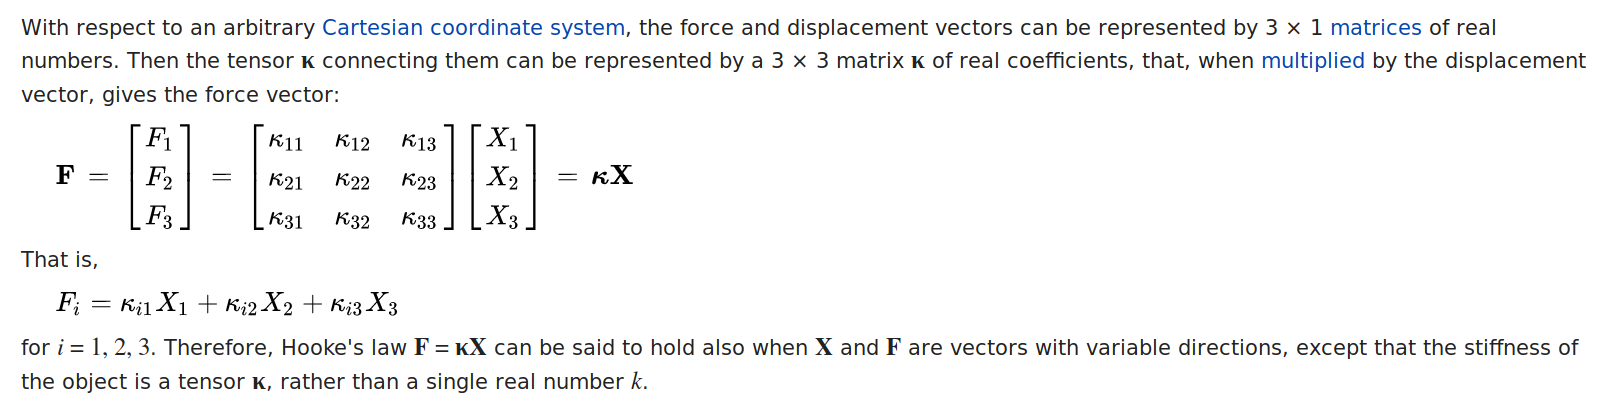
\includegraphics[width=.9\textwidth]{images/misc/stiffness_tensor.png}
%\caption{Loaded tendon}
%\label{fig:figura1}
\end{figure}

\section{Methods}

\subsection{Setup}

For the setup, I used a triple-beam balance as a way to apply force while retaining a vertical
angle. I hot-glued a pumpkin awl to the bottom of the plate and put standard weights on top of of
the scale. This caused the awl to contact the surface of the finger, and the finger would then
deflect. 

\begin{figure}[H]
\centering
%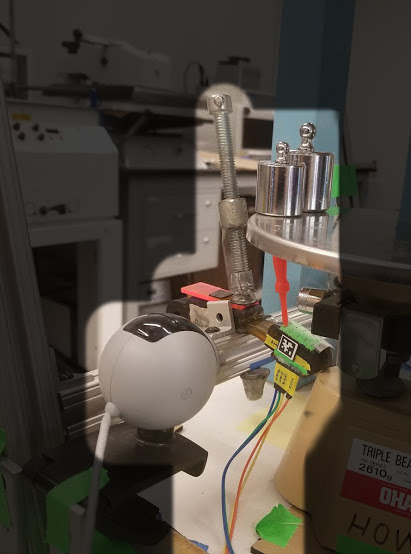
\includegraphics[width=.3\textheight]{images/setup/webcam-edit.jpg}
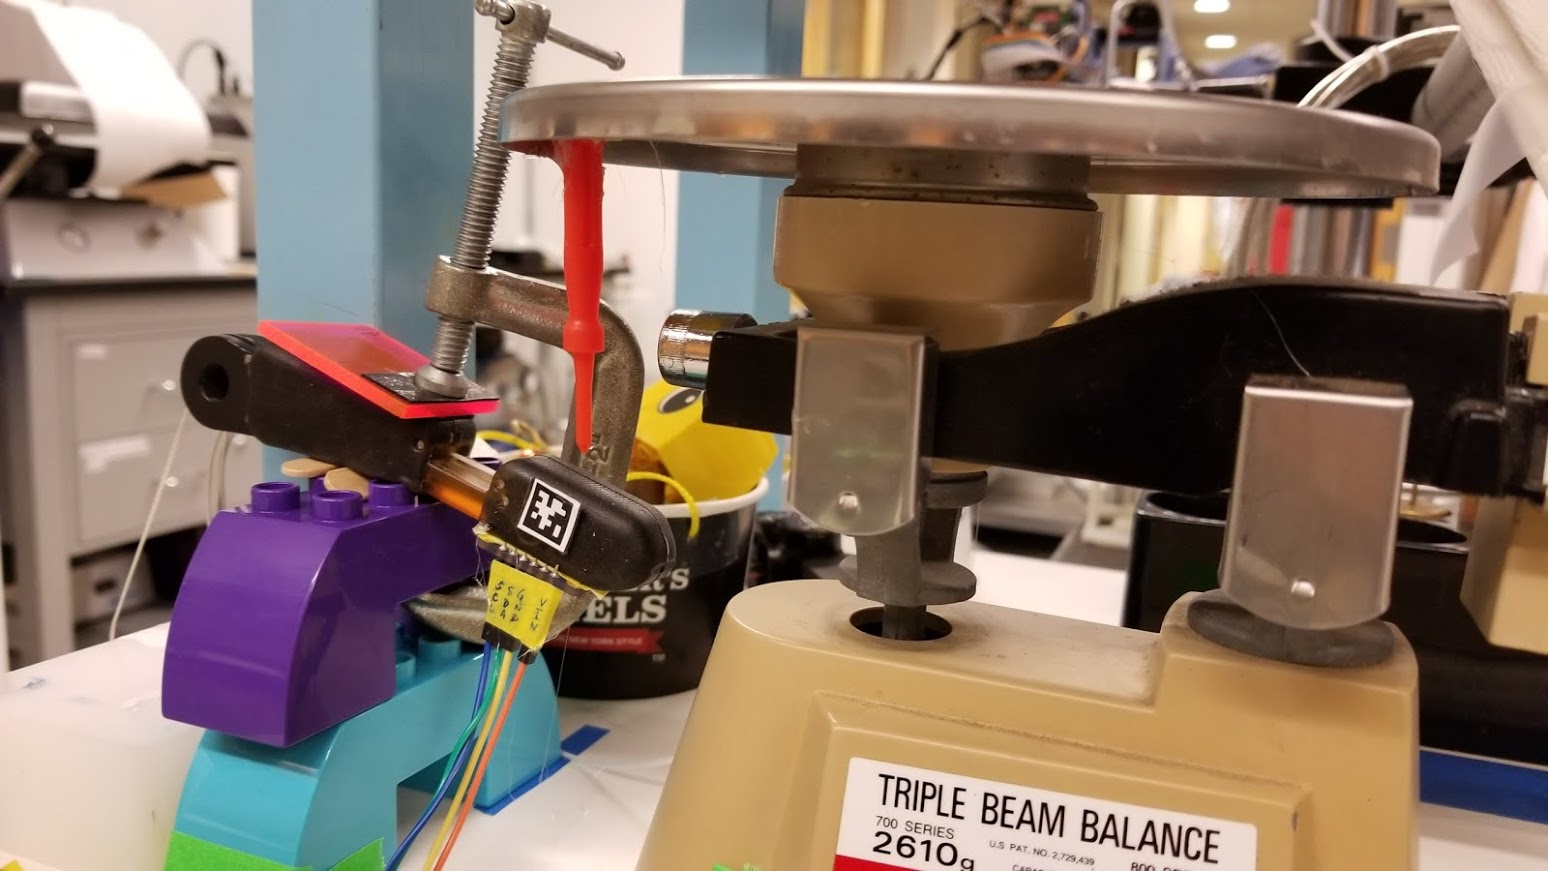
\includegraphics[width=.3\textheight]{images/setup/closeup.jpg}
%\caption{Loaded tendon}
%\label{fig:figura1}
\end{figure}

In the 1D case, I simply placed a ruler behind the finger and used a webcam to take
pictures. By mapping pixel counts to millimeters, I could then estimate the deflection of the
finger. The linear fit from these very imprecise measurements proved linear enough that I then
relied on the IMU going forward and skipped the step (which should be completed eventually) of
characterizing the accuracy of the IMU versus a gold standard, such as a stereo camera (the
Microntracker available in lab) or other methods (such as using Apriltags with a calibrated webcam). 

I then created a grid of 15 points on the finger. For each of the 15 points, I applied several known
amounts of force, with three samples at each force-point combination. Each sample consisted of a
"zero" measurement pre-contact and a measurement post-contact. In post-processing, I then subtracted
the two to obtain my final sensor data.

\begin{figure}[H]
\centering
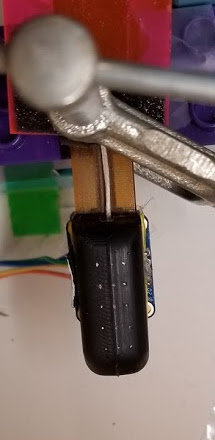
\includegraphics[width=.15\textheight]{images/setup/grid2.jpg}
%\caption{Loaded tendon}
%\label{fig:figura1}
\end{figure}


Complications arose from the limited travel of the triple beam balance, which meant I could only
measure small deflections (initially on the order of 4 mm; after discovering that I could take the
end stop off the back edge of the triple beam balance, about 10mm). At the tip of the finger, I
could only less than a hundred grams of "force" (about 1 N), while 4N is a normal amount of force
applied by humans to grasp things. This remained a source of frustration throughout the data
collecting and ate up many hours of adjusting the experimental setup. 

I glued an IMU to the undersid of the finger. The IMU I used was the Bosch BNO055 sensor. A breakout
was available from adafruit.com for \$35, which is relatively inexpensive.  I chose this sensor not
only for the built-in processing, and also because of the extensive beginner-friendly documentation
developed by Adafruit for all of its products. It was recommended to me by 
%(person) 
at Right Hand Robotics, which is a spinoff of this lab.

\begin{figure}[H]
\centering
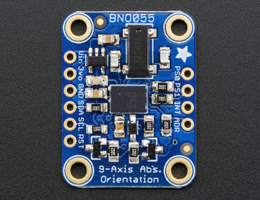
\includegraphics[width=.3\textwidth]{images/setup/bno055.png}
%\caption{Loaded tendon}
%\label{fig:figura1}
\end{figure}

\textit{"Bosch is the first company to get this right by taking a MEMS accelerometer, magnetometer and
    gyroscope and putting them on a single die with a high speed ARM Cortex-M0 based processor to digest
    all the sensor data, abstract the sensor fusion and real time requirements away, and spit out data
you can use in quaternions, Euler angles or vectors." (source: adafruit.com)}

\begin{figure}[H]
\centering
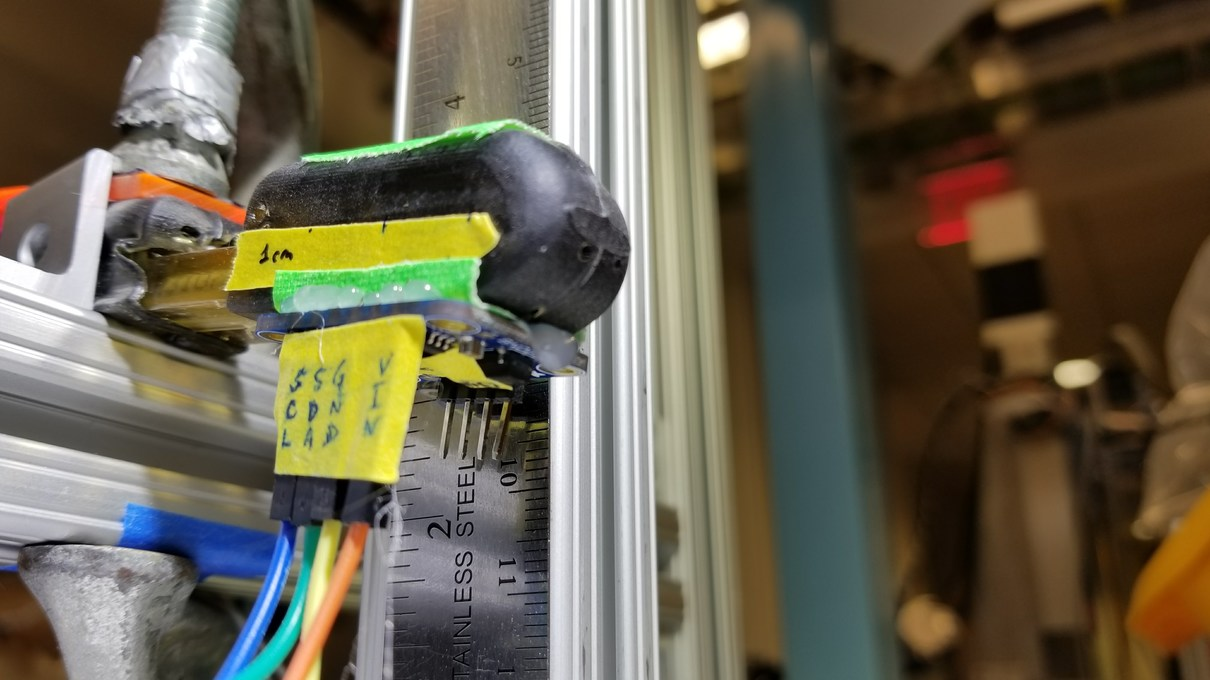
\includegraphics[width=.5\textwidth]{images/setup/IMU.jpg}
%\caption{Loaded tendon}
%\label{fig:figura1}
\end{figure}

I also attached an apriltag (which looks like a QR code) and a micontracker tag (which has a
checkerboard like cross), both of which can simply be printed out on paper, and calibrated the
webcam for use with the Apriltag C++ script. Although I have collected mictrontracker and apriltag
data for comparing to the IMU deflection data, I have not had a chance to analyze this data yet,

Additionally, the IMU acclerometer would consistently refuse to calibrate if the sensor did not
start parallel to the ground. The significant slope of the finger versus the clamp and 90 degree
angle of the 80/20 meant that I had to approximate a slanted 80/20 setup by increasing the degrees
of freedom on the L brackets (removing t-nuts). This led to a lot of worry on my part about the
creakiness and variability in the data collection as I could not guarantee angle consistency,
although in retrospect this is almost completely mitigated by the fact that I am zeroing before
every reading. 

\begin{figure}[H]
\centering
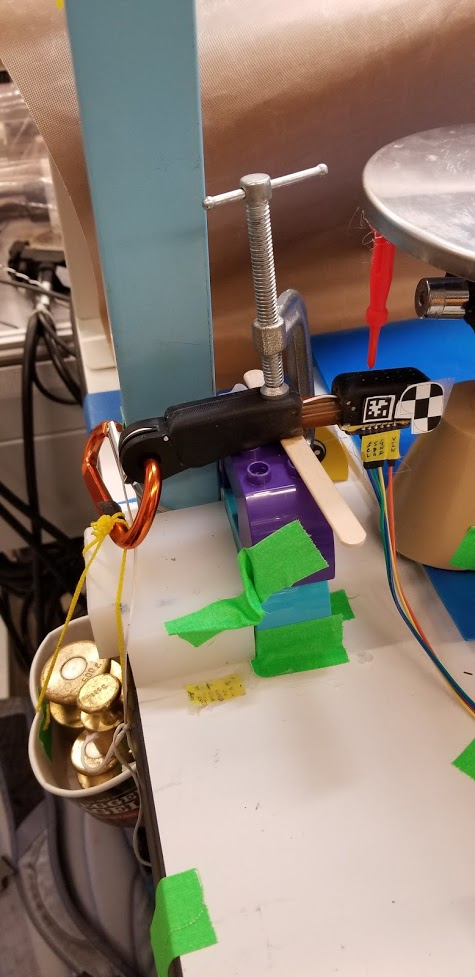
\includegraphics[width=.15\textheight]{images/setup/leveling.jpg}
%\caption{Loaded tendon}
%\label{fig:figura1}
\end{figure}

In order to apply load to pull on the tendon and change the stiffness of the finger, I decided on a
simple setup where I hung a weight from the tendon.

\begin{figure}[H]
\centering
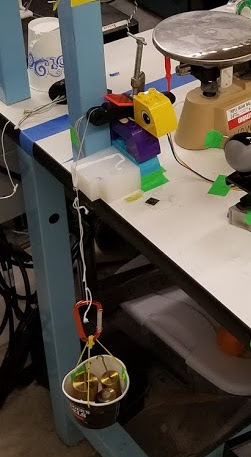
\includegraphics[width=.15\textheight]{images/setup/loading.jpg}
%\caption{Loaded tendon}
%\label{fig:figura1}
\end{figure}%

As I progressed, I trended toward collecting coarser and coarser data as I grew confident
that measurements still provided enough data for me to see overall trends in the data
(such as the linearity of the data). I shifted from 2g increments, to 20g, and in the end 50g
increments. This meant that for the finger when stiffness was applied, I had to change the setup so
that the finger started at an angle and became parallel to the floor when load was applied to the
tendon. After my deep grievances with producing angles on the 80/20 setup, I decided to use legos
with popsicle stick props on one end in order to produce the correct angles.

Finally, I discovered at the very end that I could calibrate the scale to have a constant force
offset. Thus, instead of collecting a zero measurement with the tip starting just above the surface,
which meant that I had to wait for the oscillations to settle, I could put an offset which made the
scale keel all the way to up when the weight was removed. This made zero measurements 2-3x
faster, which reduced the cognitive load to remember which measurement I was at, which both reduced
data cleanup and needing to recollecting data. This led to significant time savings.

\begin{figure}[H]
\centering
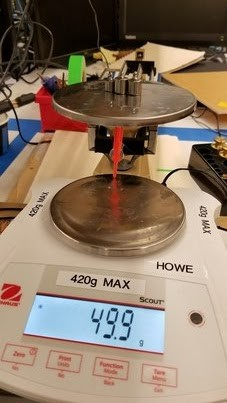
\includegraphics[width=.1\textheight]{images/setup/scale_calibration.jpg}
\caption{Scales and more scales: calibrating the weight applied with the triple beam balance using an electronic scale }
%\caption{Loaded tendon}
%\label{fig:figura1}
\end{figure}


\begin{figure}[H]
\centering
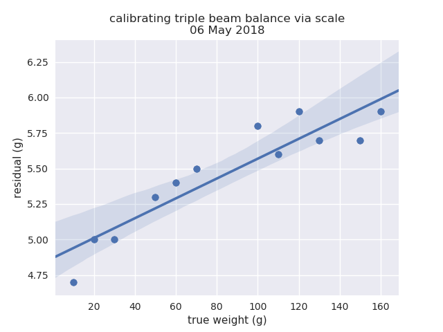
\includegraphics[width=.6\textwidth]{images/setup/scale_calibration_graph.png}
\caption{Scale calibration graph, with nominal offset of 5g. I observed that the offset is not
constant and increases with increasing load.}
%\label{fig:figura1}
\end{figure}


%TODO pictures

\section{Data Analysis}\label{sec:analisedosdados}

\subsection{Loaded tendon data}

For the final dataset, I collected data in 50g intervals at 2 y locations and 3 x locations on the
finger (total of 6 positions). 

First, a quick sanity check. By plotting torque versus measured theta, we see that the data follows
a linear pattern, as we would expect.

\begin{figure}[H]
\centering
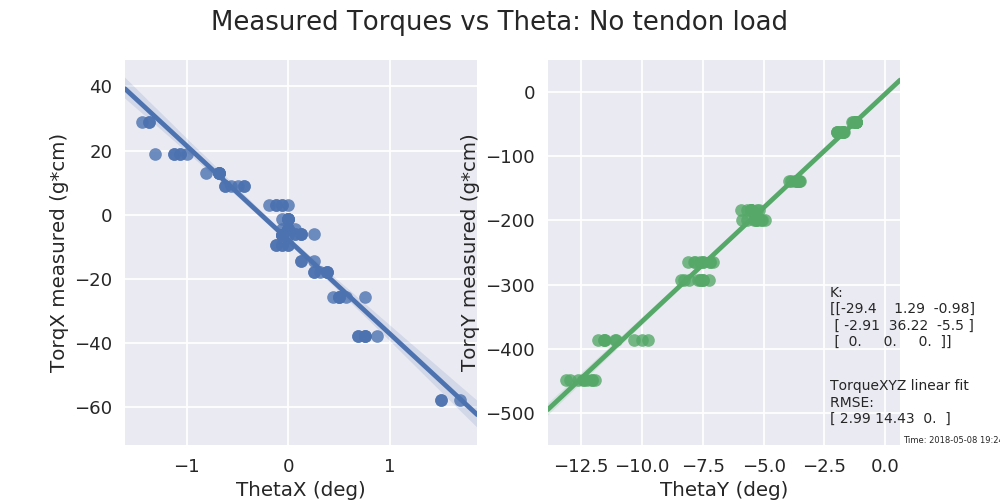
\includegraphics[width=\textwidth]{images/stiff/torqtheta.png}
\caption{Relaxed tendon}
%\label{fig:figura1}
\end{figure}


\begin{figure}[H]
\centering
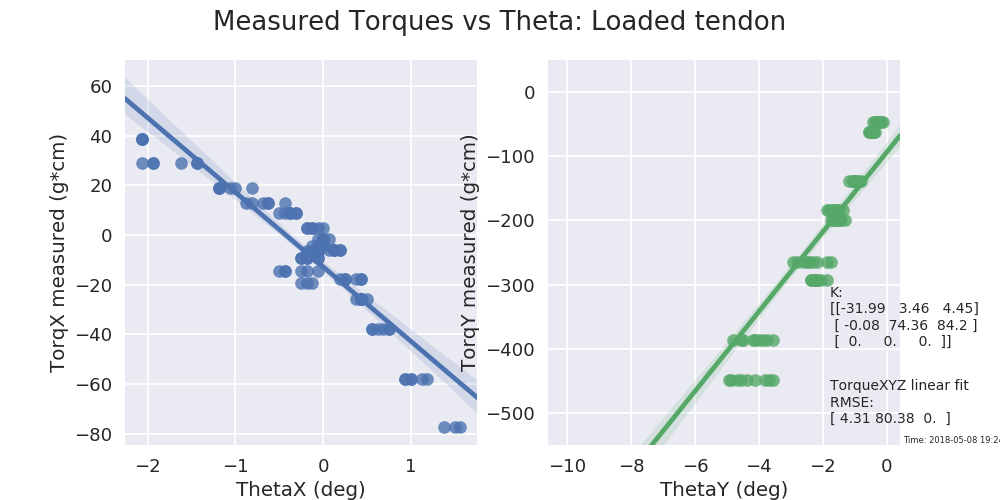
\includegraphics[width=\textwidth]{images/stiff/torqtheta_loaded.png}
\caption{Loaded tendon}
%\label{fig:figura1}
\end{figure}

Additionally, we may see that we have properly fitted our data with a K matrix by comparing our
newly created torque estimates, versus the original measurements. The datapoints do not fall
precisely on a line because the K matrix and fit is in three-dimension. In picking a single
dimension to plot, the projection results in datapoints that are not linear in one dimension despite
a linear fit overall.

\begin{figure}[H]
\centering
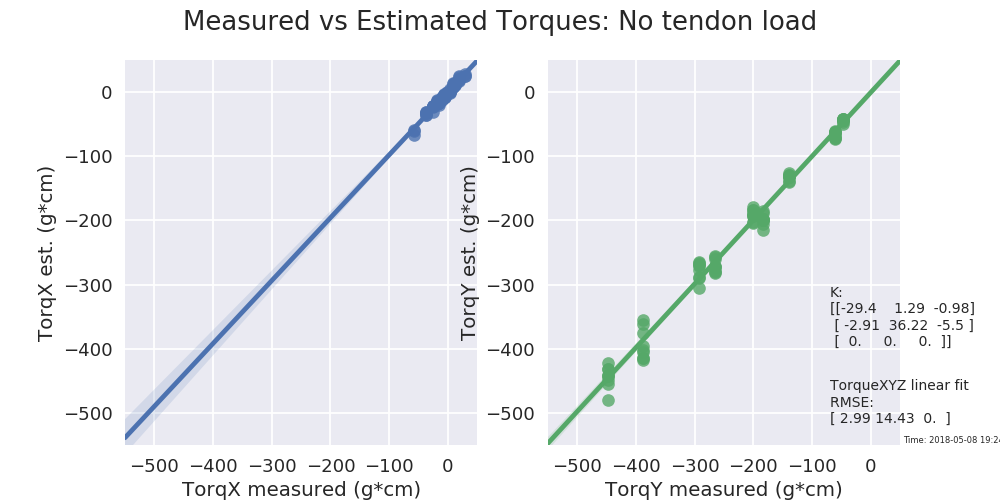
\includegraphics[width=\textwidth]{images/stiff/torqsanity.png}
\caption{Relaxed tendon}
%\label{fig:figura1}
\end{figure}

\begin{figure}[H]
\centering
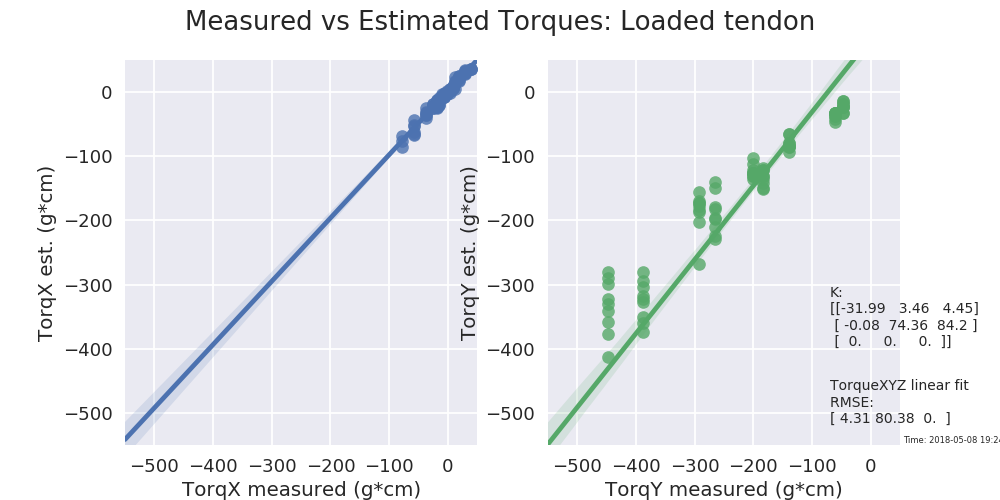
\includegraphics[width=\textwidth]{images/stiff/torqsanity_loaded.png}
\caption{Loaded tendon}
%\label{fig:figura1}
\end{figure}



Next we can look at the residuals. Based on the previous experiment, I was expecting to see a linear
relationship in the residuals between ThetaY and TorqueY. However, I did not see any such
relationship in the relaxed case, which should have most closely matched the data in the previous
experiment. 

\begin{figure}[H]
\centering
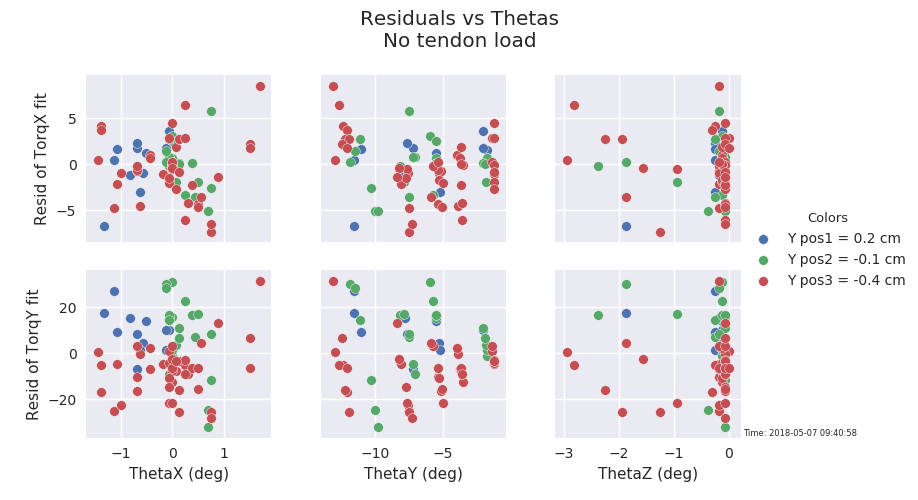
\includegraphics[width=.9\textwidth]{images/stiff/GOODResid_vs_Theta.png}
\caption{Relaxed :tendon}
%\label{fig:figura1}
\end{figure}

A pattern did appear in the loaded case. Further investigation will be required.

\begin{figure}[H]
\centering
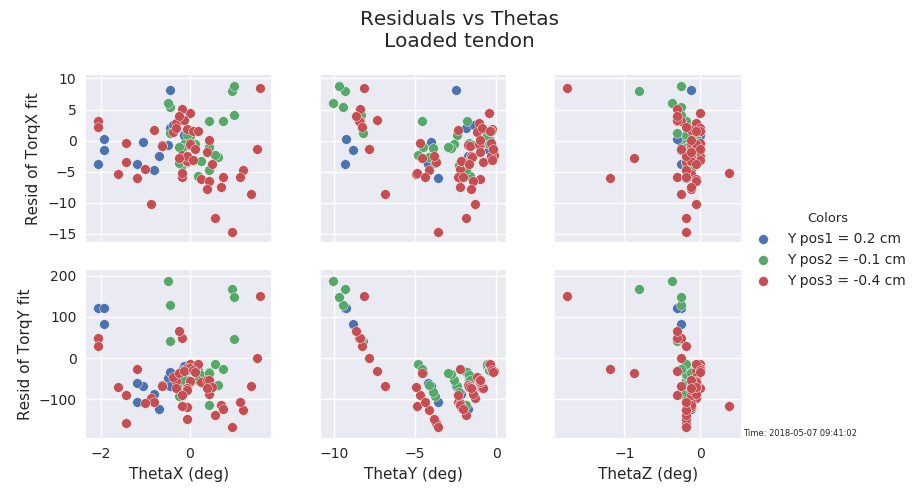
\includegraphics[width=.9\textwidth]{images/stiff/GOODResid_vs_Theta_loaded.png}
\caption{Loaded tendon}
%\label{fig:figura1}
\end{figure}

Patterns in the thetaZ may be ignored as it was not used in the fit (zeroed out by zero for Force)

\begin{figure}[H]
\centering
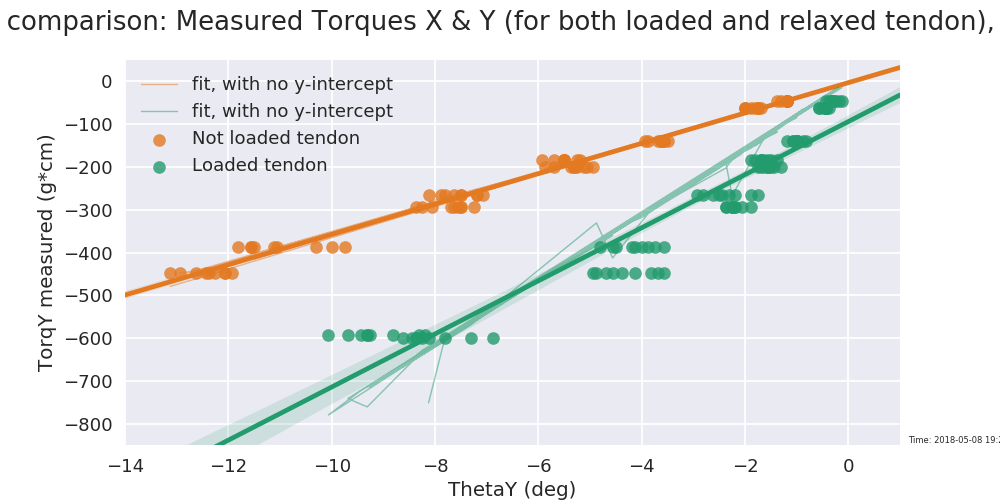
\includegraphics[width=.9\textwidth]{images/stiff/StiffnessComparison.png}
\caption{Loaded case shown in green, relaxed tendon shown in orange. This graph shows that the
loaded tendon is stiffer (slope is steeper), as we expect. Both models seem mostly linear, but it's
possible that in the loaded case, the fit is more exponential. Note that physically the model must
go through the y-intercept, and I have graphed the actual fit used to calculated residuals in light
green (albeit for a nonlinear fit). The dark green line is plotted due to limitations in my plotting
library}
%\label{fig:figura1}
\end{figure}

\subsection{Initial data (relaxed tendon only)}

\begin{figure}[H]
\centering
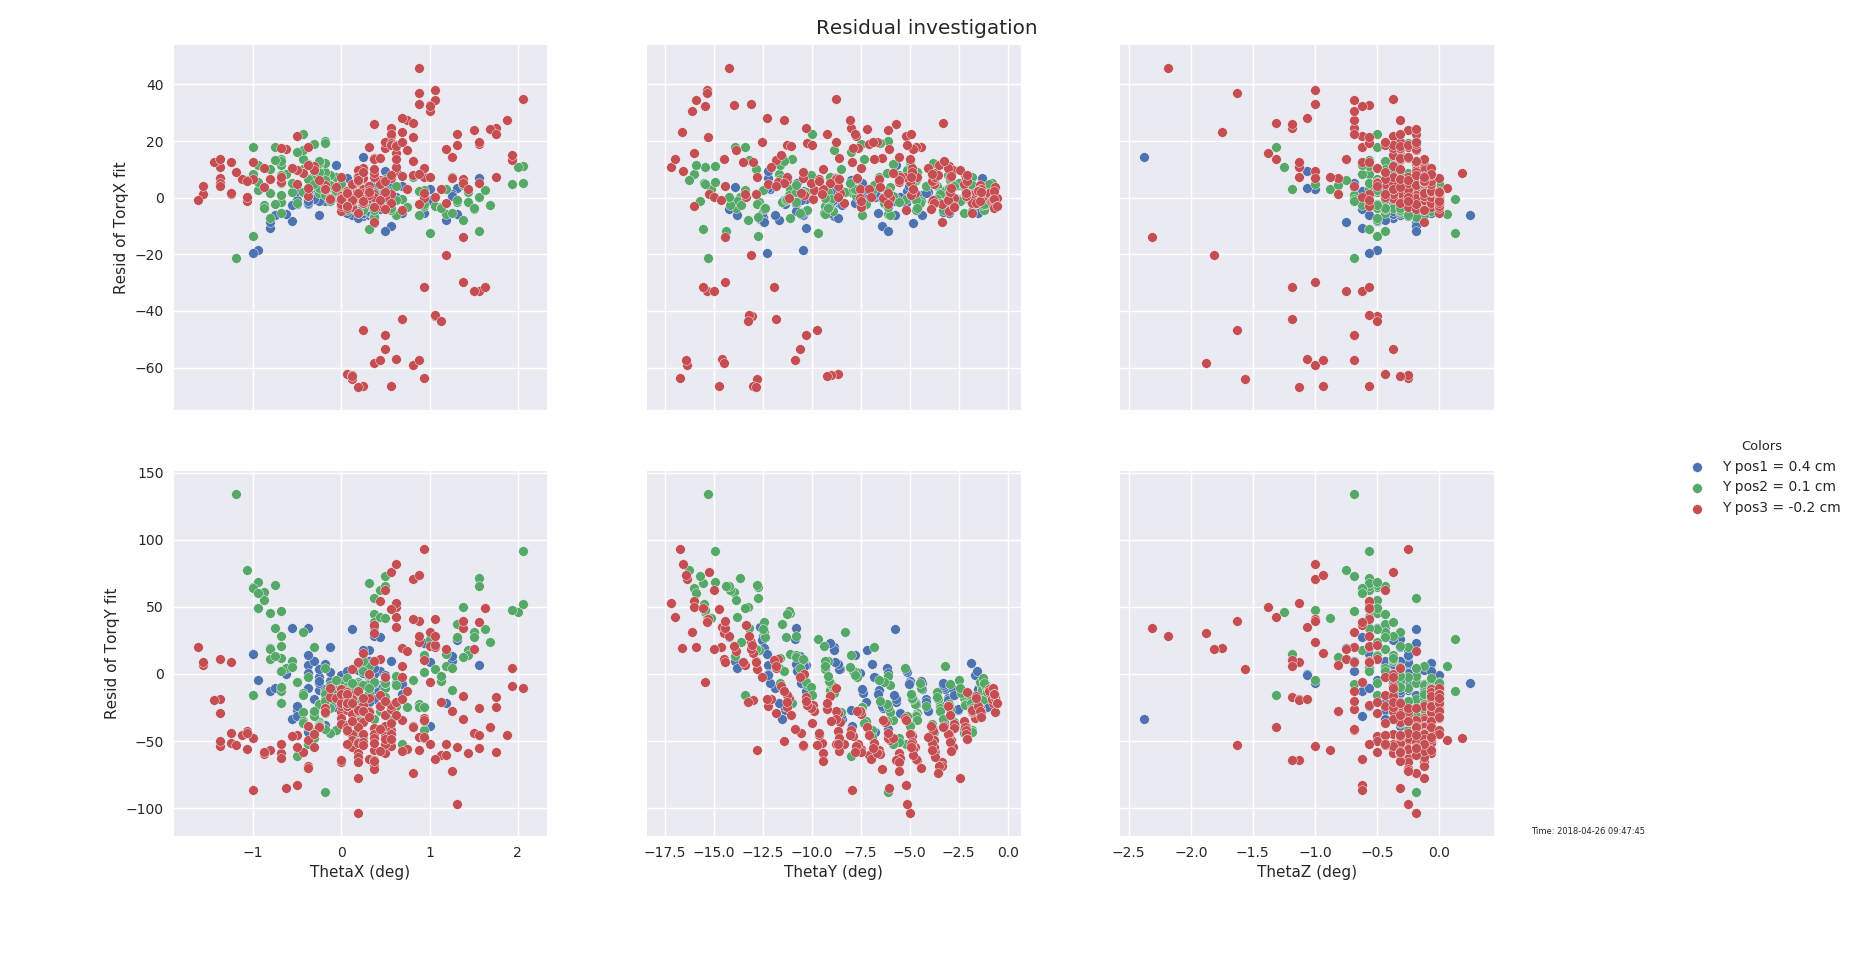
\includegraphics[width=.9\textwidth]{images/round1/LinearResid_thetaY.png}
%\caption{Loaded tendon}
%\label{fig:figura1}
\end{figure}

\begin{figure}[H]
\centering
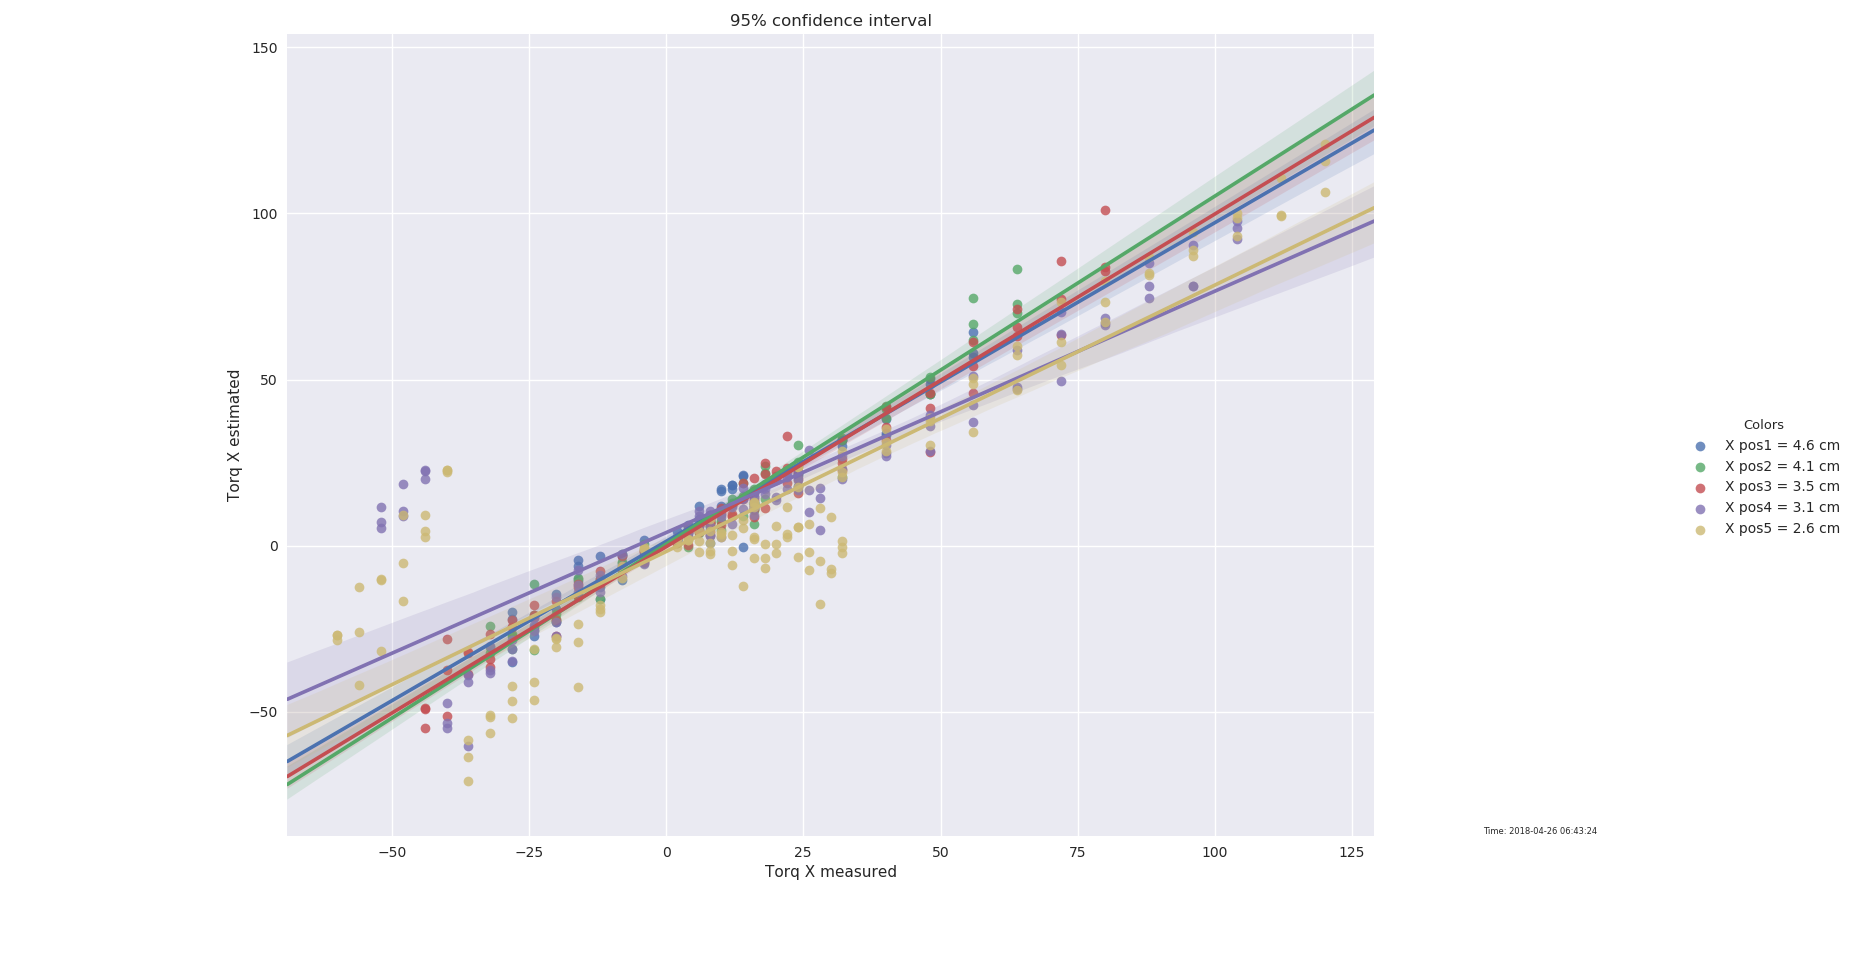
\includegraphics[width=.9\textwidth]{images/round1/TorqX_hueX.png}
%\caption{Loaded tendon}
%\label{fig:figura1}
\end{figure}

\begin{figure}[H]
\centering
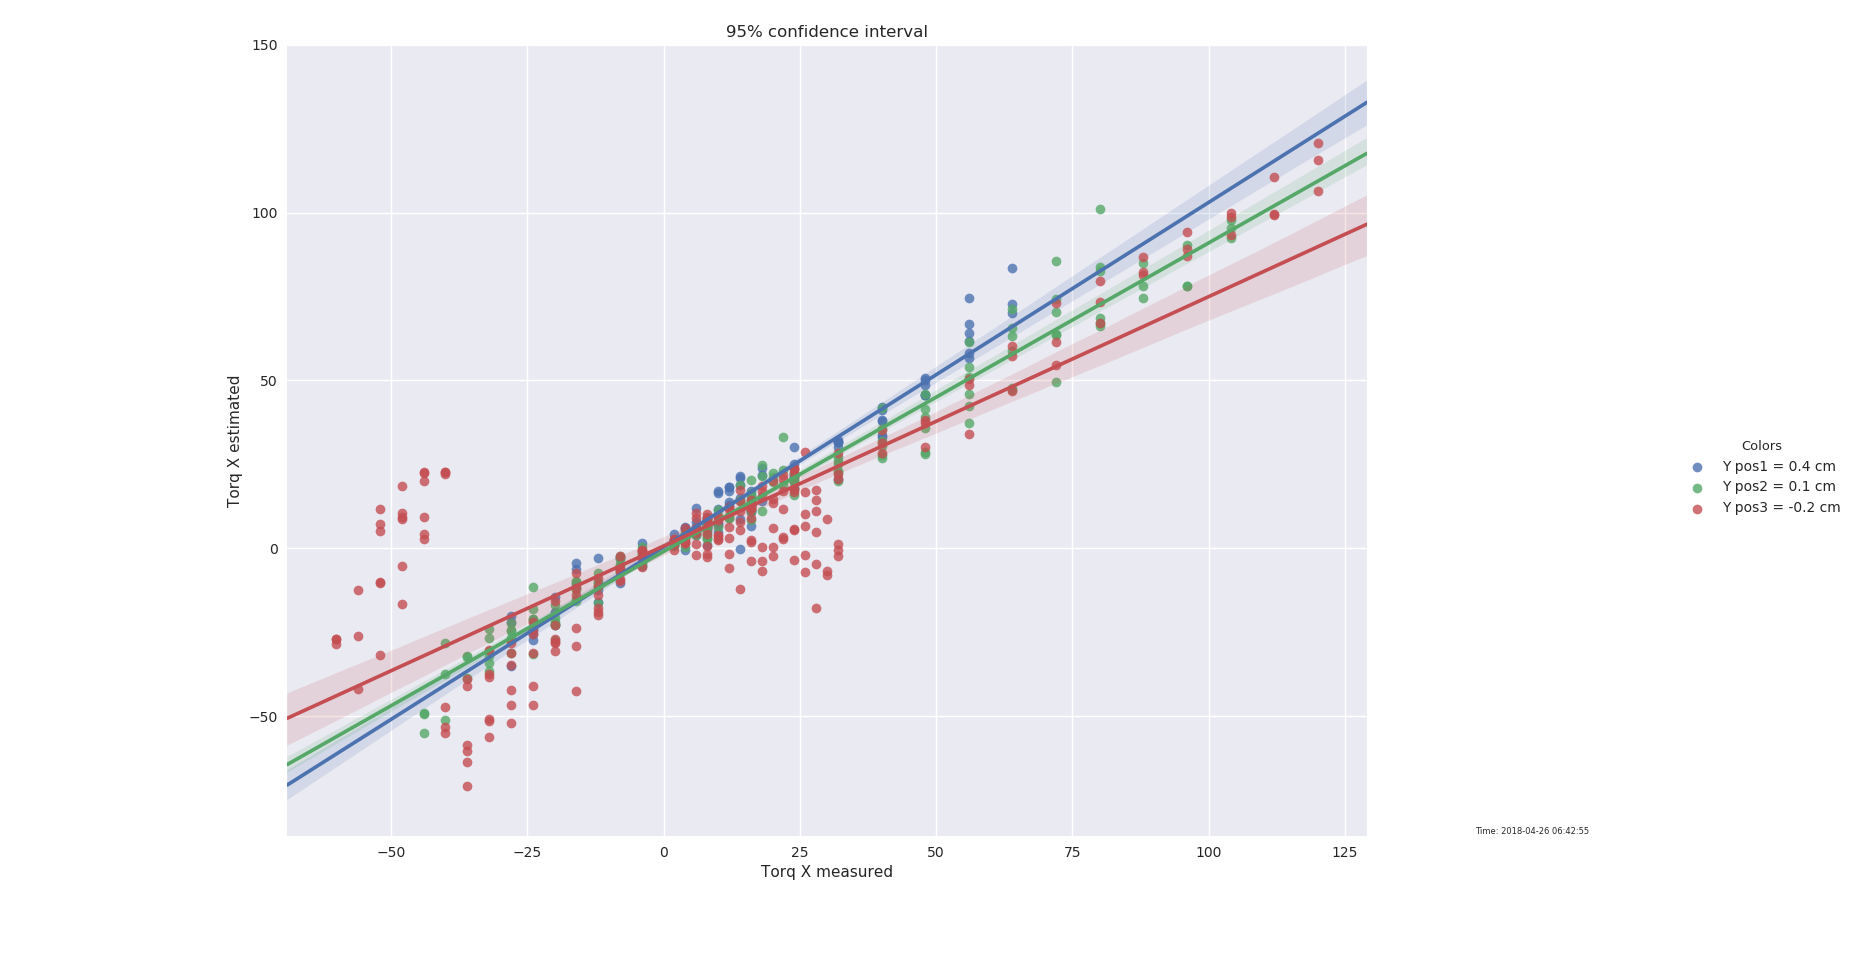
\includegraphics[width=.9\textwidth]{images/round1/TorqX_hueY.png}
%\caption{Loaded tendon}
%\label{fig:figura1}
\end{figure}


\begin{figure}[H]
\centering
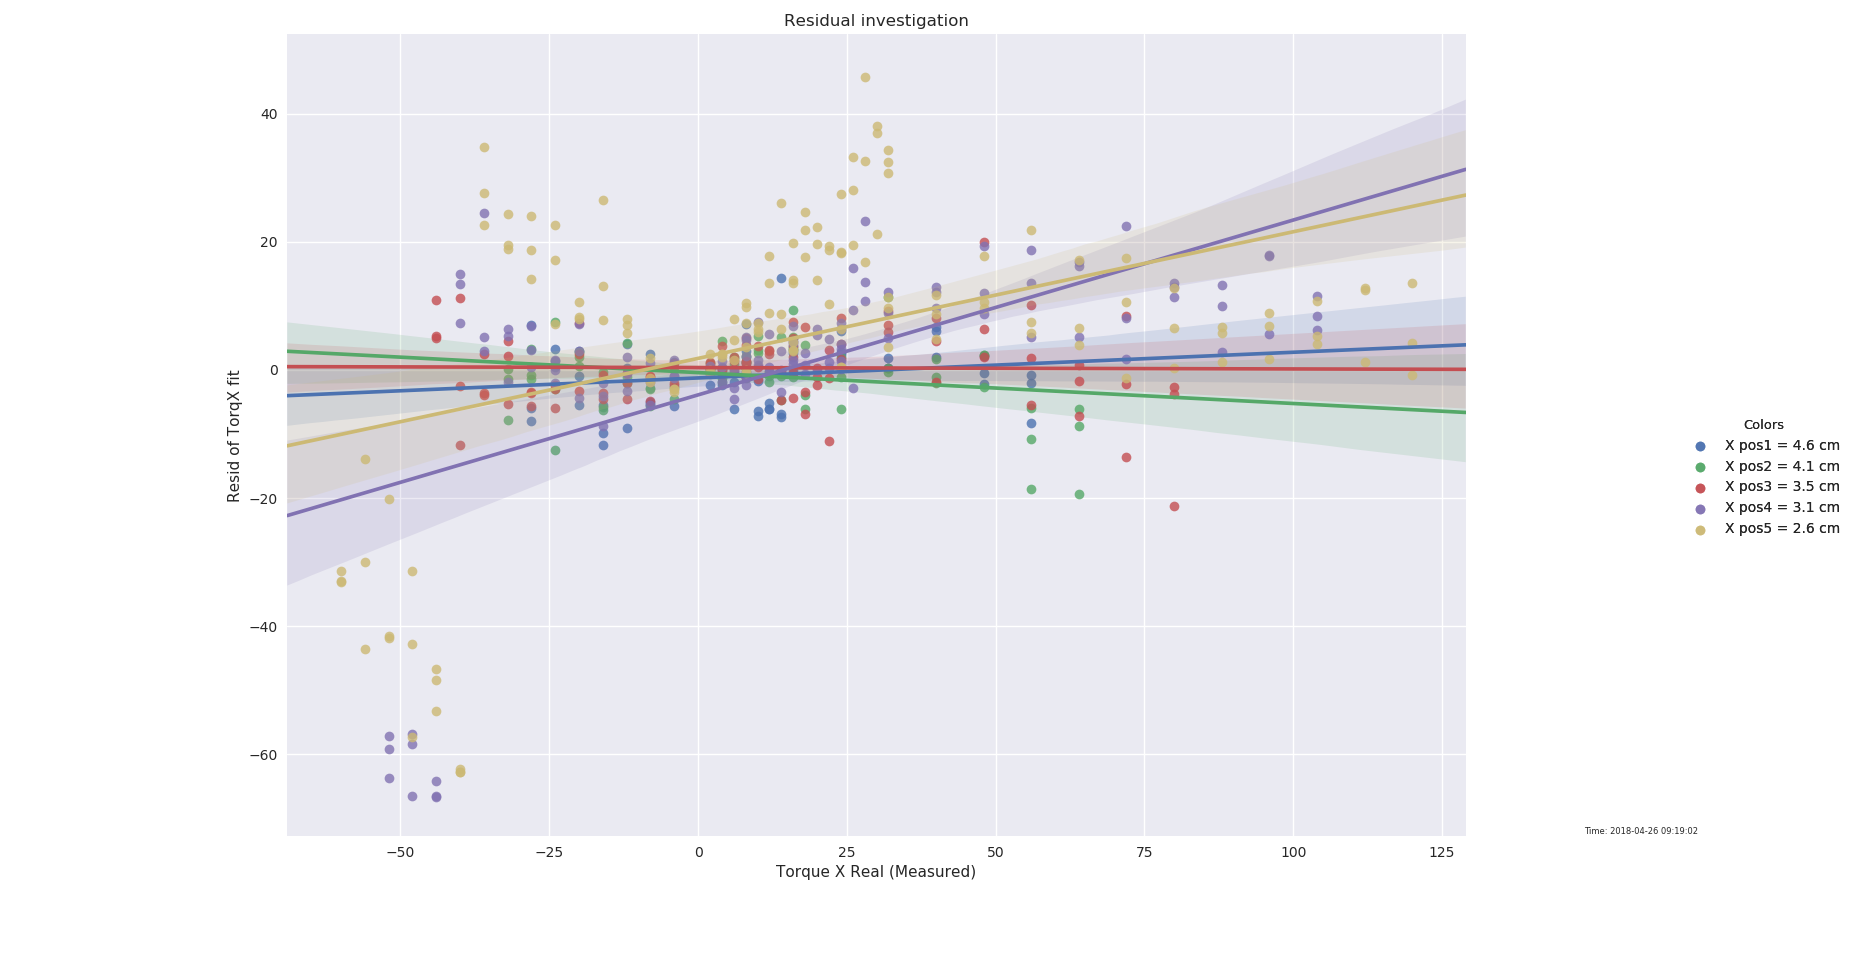
\includegraphics[width=.9\textwidth]{images/round1/ResidX_hueX.png}
%\caption{Loaded tendon}
%\label{fig:figura1}
\end{figure}

%\begin{figure}[H]
%\centering
%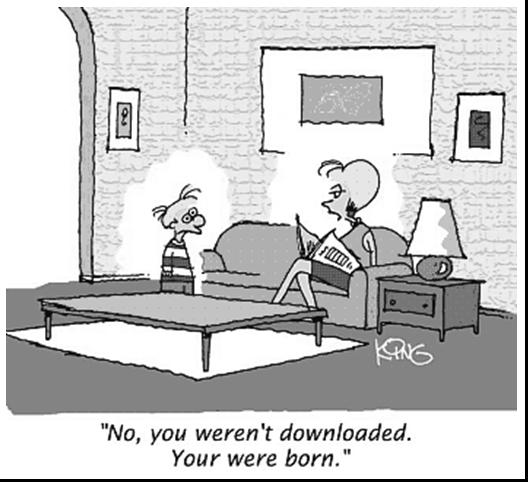
\includegraphics[width=.3\textwidth]{fig1.jpg}
%\caption{Exemplo de figura}
%\label{fig:figura1}
%\end{figure}

\subsection{1D case}

In the 1D case I simply took pictures of the finger against a ruler in order to measure angular deflection. 

\begin{figure}[H]
\centering
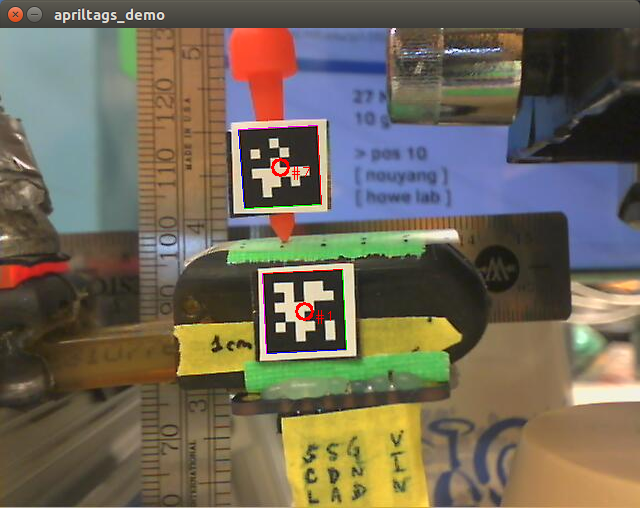
\includegraphics[width=.3\textwidth]{images/1d/zero.png}
\caption{Zeroed}
%\label{fig:figura1}
\end{figure}

\begin{figure}[H]
\centering
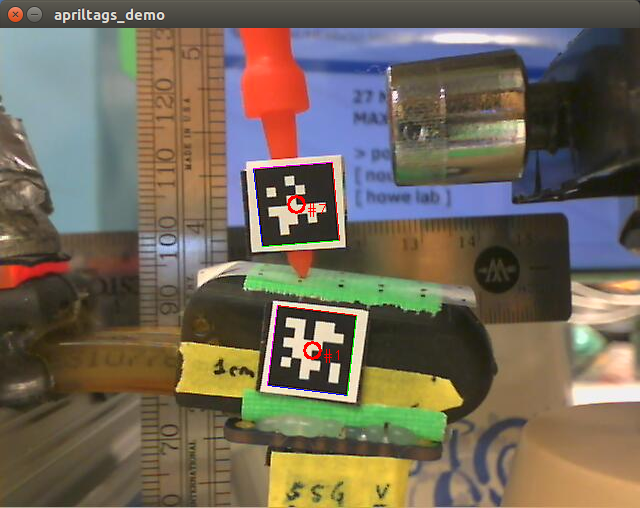
\includegraphics[width=.3\textwidth]{images/1d/weighted.png}
\caption{With pressure applied}
%\label{fig:figura1}
\end{figure}

%\begin{figure}[H]
%\centering
%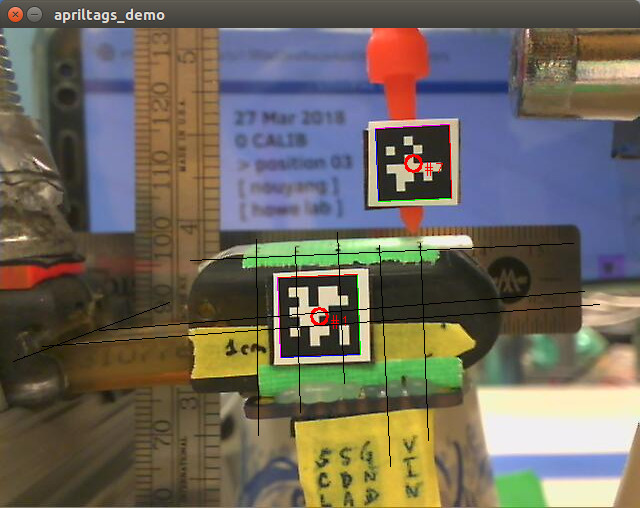
\includegraphics[width=.3\textwidth]{images/1d/torque_calc.jpg}
%\caption{Drawing lines to estimate neutral axis}
%%\label{fig:figura1}
%\end{figure}

\subsection{Attempted fit improvements}
%Nesta seção, o aluno descreve o efetivo procedimento metodológico adotado e aponta os resultados da pesquisa. Na análise de dados, é  aconselhável o uso de tabelas, figuras, linhas de códigos etc para representar os resultados do estudo.

%As Tabelas, Quadros e Figuras, assim como as legendas de Tabelas, Quadros e Figuras devem estar centralizadas se conterem apenas em uma linha (Figura~\ref{fig:figura1}), caso contrário devem estar tabuladas em 0.8cm em ambas as margens, como mostra a Figura~\ref{fig:figura2}. 

%\begin{figure}[H]
%\centering
%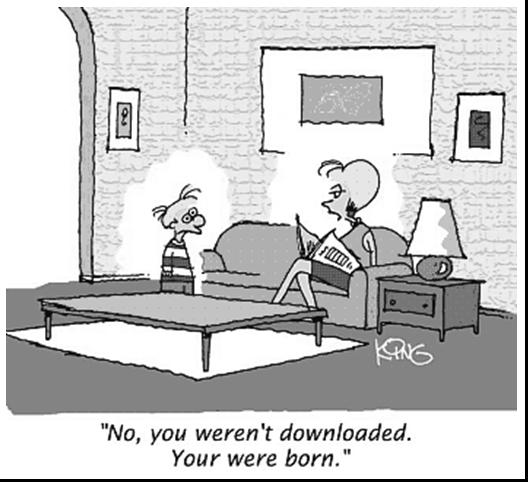
\includegraphics[width=.3\textwidth]{fig1.jpg}
%\caption{Exemplo de figura}
%\label{fig:figura1}
%\end{figure}

%As legendas devem ser escritas na fonte “Helvetica”, Tamanho 10pts, negrito, com espaço de 6pts antes e depois de cada legenda. Sempre que possível, procure colocar a figura delimitada por um quadro (Figura~\ref{fig:figura1} e Figura~\ref{fig:figura2})

%\begin{figure}[!ht]
%\centering
%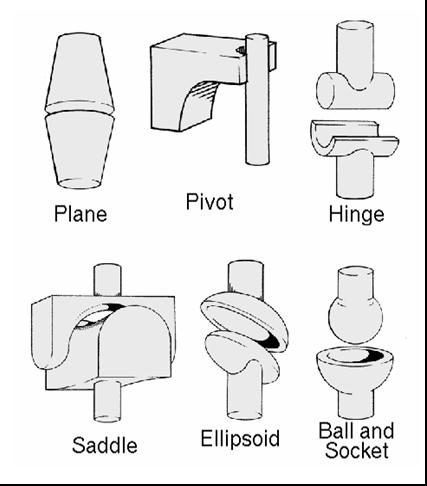
\includegraphics[width=.2\textwidth]{fig2.jpg}
%\caption{Essa figura foi referenciada na Seção~\ref{sec:analisedosdados}.}
%\caption{Fonte: SBC.}
%\label{fig:figura2}
%\end{figure}

%Em tabelas, tente evitar o uso de fundos coloridos ou preenchidos, assim como linhas duplas na borda, ou linhas desnecessárias. Quando \cite{knuth:84} relatar dados empíricos, não faça uso de mais dígitos decimais do que o necessário. A legenda da tabela deve ser colocada antes da tabela (veja Tabela 1) e a fonte usada na legenda deve ser Helvetica, tamanho 10pts, negrito, com 6pts de espaço antes e depois de cada legenda.

%\begin{table}[!ht]
%\centering
%\caption{Exemplo de tabela de 3 colunas e 2 linhas}
%\label{tab:exTable1}
%\smallskip
%\begin{tabular}{l c c}
%\hline
%& Value 1 & Value 2\\[0.5ex]
%\hline
%&&\\[-2ex]
%Case 1 & 1.0 $\pm$ 0.1 & 1.75$\times$10$^{-5}$ $\pm$ 5$\times$10$^{-7}$\\[0.5ex]
%\hline
%&&\\[-2ex]
%Case 2 & 0.003(1) & 100.0\\[0.5ex]
%\hline
%\end{tabular}
%\end{table}
\section{Sensor Design}


MLP
\begin{figure}[H]
\centering
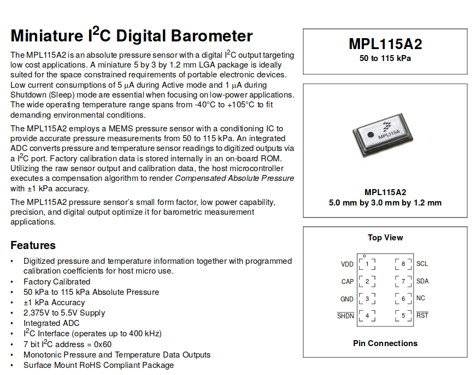
\includegraphics[width=.5\textwidth]{images/sensor/old_datasheet.png}
%\caption{Loaded tendon}
%\label{fig:figura1}
\end{figure}

Newer (smaller footprint)
\begin{figure}[H]
\centering
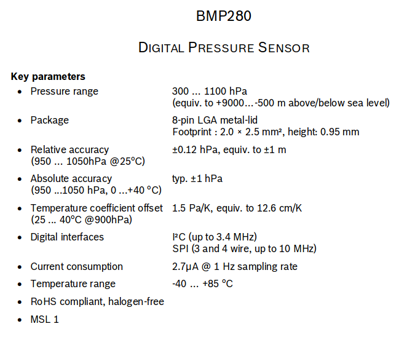
\includegraphics[width=.5\textwidth]{images/sensor/new_datasheet.png}
%\caption{Loaded tendon}
%\label{fig:figura1}
\end{figure}

Prototype
\begin{figure}[H]
\centering
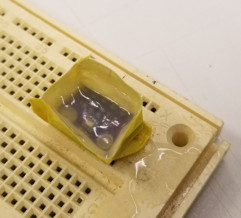
\includegraphics[width=.3\textwidth]{images/sensor/sensor.jpg}
%\caption{Loaded tendon}
%\label{fig:figura1}
\end{figure}


Prototype cured
\begin{figure}[H]
\centering
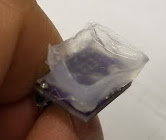
\includegraphics[width=.3\textwidth]{images/sensor/sensor2.jpg}
%\caption{Loaded tendon}
%\label{fig:figura1}
\end{figure}


I produced Arduino and python code that allowed me to view a plot in real time of the sensor data.

Additionally, I integrated the Arduino with an RGB LED strip, where if you pressed on the sensor,
more LEDs would light up.

The sensor displayed a large amount of hysteresis, which should be investigated and addressed.

This required use of a separate power supply, otherwise the Arduino would refuse to talk to the
computer (for real-time plotting) when the LED strip drew load on the 5V line.

\section{Miscellaneous}
\subsection{Time estimates}

An additional yet important thing in any project is measuring project slip in the hopes of
developing better time estimates. 

\begin{figure}[H]
\centering
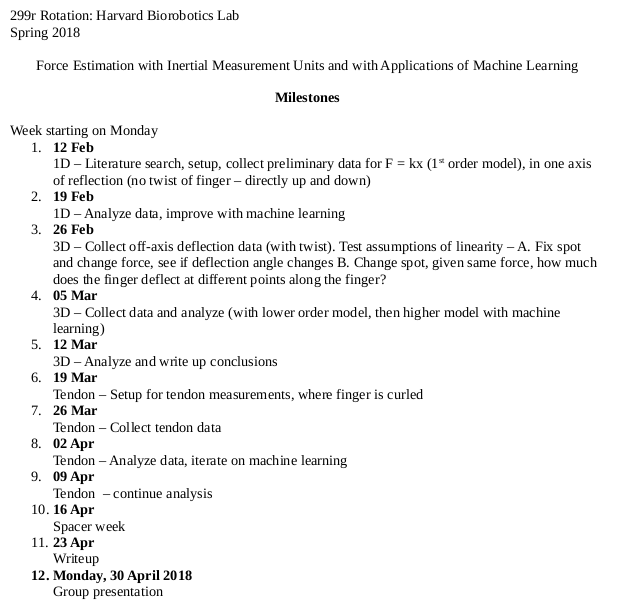
\includegraphics[width=.8\textwidth]{images/misc/timeline.png}
%\caption{Loaded tendon}
%\label{fig:figura1}
\end{figure}

%TODO

\section{Knowledge}

In the process of this research, I learned about how accelerometers are calibrated, which I found
very interesting (although ultimately, thanks to the built-in sensor fusion and calibration routines of the BNO055
sensor, I did not need to write my own calibration routines). The common presence of the gravity
vector across meaurements at diffent angles makes this calibration possible.

I learned the most about exploratory statistical data analysis. Where previously I had not even
heard of residuals (only scalar measurements such as mean-square-error), I learned about how they
could be compared to a horizontal basis against which they would be randomly distributed assuming
random noise around a proper physical model.

Finally, I learned more about the I2C and SPI protocols for receiving (and writing) to multiple
sensors. I began work on creating a custom printed circuit board to create a 3x4 array of sensors,
and decided to switch and learn to use a newcomer in the PCB design space, which has CERN support: the free and open-source
KiCAD tool.

\section{Conclusions}

The stiffness of the finger was remarkably linear, which meant that machine learning and higher
order terms had little to contribute to improving the fit between measure theta deflections and
force estimates.

However, I was only able to apply relatively small loads to the finger. It's possible that with
large loads, the stiffness becomes less linear, in which case linear fit residuals may become more
prominent or structured. If this were the case, machine learning approaches might have more to
contribute to the force estimates. As it were, the data I collected did not benefit much from the
addition of non-linear models fitted with machine learning techniques such as random forests.

Most crucially, Qian demonstrated to me the process by which grasps fail. By observing the grasping,
I discovered that when the tendon was pulled taught (as needed to grasp anything), the y-axis was now
now the stiffest axis! Thus, characterizing the finger with no tendon load applied and primarily in
the y-axis direction, while a great learning experience, does not generalize at all to practice and becomes a
toy example.

Additionally, the finger relied extensively on mechanical mechanism intelligence (as opposed to full
actuated parallel grippers, commonly used in computer science labs).  I saw that complete failures
tended to occur because the finger had failed to detect contact when contact had already occured.
This suggests the better instrumentation of the finger is critical. The IMU by itself can only
suggest contact force, and the tactile sensors are needed to tell contact location. To evaluate the
contribution of the IMU to force estimates and not just torque estimates, we must build better
location sensors than the current 1x4 array.

%Referências bibliográficas devem ser utilizadas dentro de um estilo uniforme e não ambíguo. A SBC sugere os seguintes formatos para referências: \cite{knuth:84}, \cite{boulic:91}, e \cite{smith:99}.

%\bibliographystyle{sbc}
%\bibliography{sbc-template}

\subsection{Future Work}

The microntracker should be used to evaluate the IMU. Evaluating the use of Apriltags with the
microntracker would help reproducibility by others (or future grad students), as webcams are cheap
and readily available, and documentation for apriltags is freely available online.

Additionally, a full sensor array on a custom PCB, manufactured into a finger unit, should be
developed and characterized. By collecting data and then fusing this with the IMU data, we could
physically evaluate the grasp stability preductions, producing an important tie between theory and
practice to ensure the two complement each other. The important of this has been mentioned above.

\appendix

\section{Section in Appendix}

\subsection{Apriltags}
I decided to investigate apriltags, which helped me refresh on my knowledge of C++. I struggled to
find an appropriate ROS driver, and ultimately was able to get the C++ working (despite some issues
with the openCV version on my laptop) with the help of Patrick from Prof. Kuindersma's lab.

Example data output
\begin{ttlisting}
2 tags detected: 
Id: 1 (Hamming: 0) distance=0.079741m, x=0.000532, y=0.006102, z=-1.487915, yaw=-0.134615, pitch=0.071828, roll=-0.041146
Id: 7 (Hamming: 0) distance=0.079741m, x=0.000532, y=0.006102, z=-1.487915, yaw=-0.134615, pitch=0.071828, roll=-0.041146
14.9312 fps
\end{ttlisting}

\begin{ttlisting}
nrw@earlgrey:~/projects/apriltags$ vi CMakeLists.txt 
    (line 14) find_package(OpenCV 2.4.9.1 EXACT REQUIRED)
\end{ttlisting}

\begin{figure}[H]
\centering
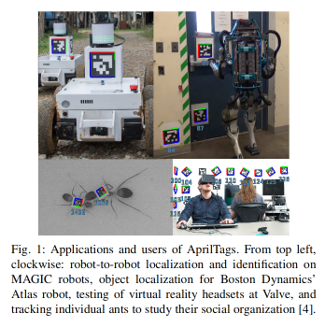
\includegraphics[width=.4\textwidth]{images/april/applications_april.png}
\caption{Loaded tendon}
%\label{fig:figura1}
\end{figure}

To calibrate the camera, I was able to find a (very!) well-documented python script online that allowed be to calibrate the camera simply by taking a few pictures of a checkerboard.

\begin{ttlisting}[language=C++,breaklines]
(venv) nrw@earlgrey:~/projects/video2calibration$ ./calibrate.py example_input/chessboard.avi calibration.yaml --debug-dir out
\end{ttlisting}

\begin{figure}[H]
\centering
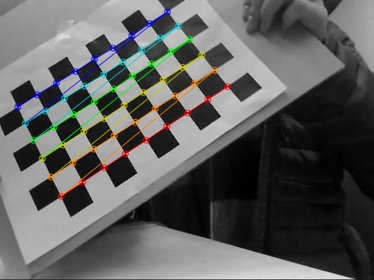
\includegraphics[width=.4\textwidth]{images/april/webcam_calibration.png}
%\caption{Loaded tendon}
%\label{fig:figura1}
\end{figure}

Using the output of the calibration script, I could then set the values in the apriltag example code
to give me (fairly accurate) estimates of the xyz location of the finger in real-world units.

\begin{ttlisting}[language=C++,breaklines]
nrw@earlgrey:~/projects/video2calibration$ ./calibrate.py ~/Videos/Webcam/2018-03-26-112657.webm calibration.yaml --debug-dir out

Performing calibration...
 RMS: 0.442700776066
 camera matrix:
 [[ 666.78668352    0.          343.73827809]
 [   0.          665.79103853  227.19081685]
 [   0.            0.            1.        ]]
 distortion coefficients:  [  6.06301194e-02  -1.94620209e-02   1.45555284e-04   1.24410189e-03
 -2.51439333e-01]
\end{ttlisting}


\begin{lstlisting}[language=C++,breaklines]
public:

  // default constructor
  Demo() :
    // default settiwgs, most can be modified through command line options (see below)
 [...excerpted section...]
    m_width(640),
    m_height(480),
    m_tagSize(0.00944), // in meters
    m_fx(667), // in pixels
    m_fy(666), //
    m_px(344), // principal point
    m_py(227),
\end{lstlisting}



\subsection{Online documentation}
I documented my work on a blog, http://orangenarwhals.github.io/, using the Hexo flatfile content
management system. I chose this because it allowed me to host for free on github, allowed for easy
version control of content, and also had an admin plugin that allowed me to drag-and-drop images,
which is crucial for documenting experiments where I have a lot of graphs. I was also able to get
Latex to work on the site so that I could have equations rendered on there.

\begin{figure}[H]
\centering
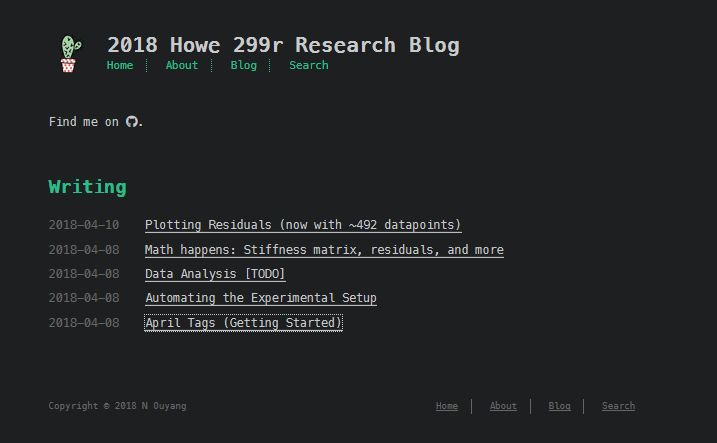
\includegraphics[width=.8\textwidth]{images/misc/blog.png}
%\caption{Loaded tendon}
%\label{fig:figura1}
\end{figure}


\begin{figure}[H]
\centering
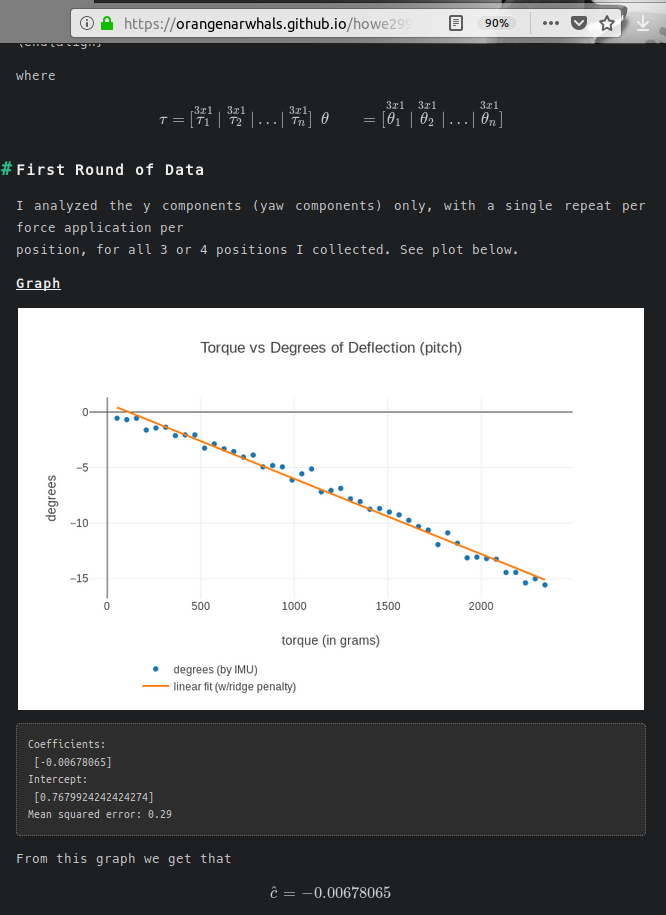
\includegraphics[width=.8\textwidth]{images/misc/blog_latex.png}
\caption{Getting latex to work was a major source of frustration.}
%\label{fig:figura1}
\end{figure}

%% References
%%
%% Following citation commands can be used in the body text:
%% Usage of \cite is as follows:
%%   \cite{key}         ==>>  [#]
%%   \cite[chap. 2]{key} ==>> [#, chap. 2]
%%

%% References with bibTeX database:

%\bibliographystyle{elsarticle-num}
%% \bibliographystyle{elsarticle-harv}
%% \bibliographystyle{elsarticle-num-names}
%% \bibliographystyle{model1a-num-names}
%% \bibliographystyle{model1b-num-names}
%% \bibliographystyle{model1c-num-names}
%% \bibliographystyle{model1-num-names}
%% \bibliographystyle{model2-names}
%% \bibliographystyle{model3a-num-names}
%% \bibliographystyle{model3-num-names}
%% \bibliographystyle{model4-names}
%% \bibliographystyle{model5-names}
%% \bibliographystyle{model6-num-names}

%\bibliography{sample}


\end{document}

%%
%% End of file `elsarticle-template-num.tex'.
